% Template para Proposta e TCC da EST/UEA -
% Padr�o para os cursos do N�cleo de Computa��o
%
% Elaborado por Ello� B. Guedes
% Adaptado da vers�o elaborada por:				%                   Jucimar Maia Jr.
%
% Vers�o beta - 08 de outubro de 2015
%
\documentclass[a4paper,titlepage,12pt]{report}


%% Pacotes elementares
\usepackage[brazil]{babel}
\usepackage[utf8]{inputenc}
\usepackage[T1]{fontenc}
\usepackage{color}
\usepackage{amsmath,amssymb,amsmath,bbm,amsfonts}
\usepackage{graphicx}
\usepackage{url}
\usepackage{booktabs} % Formatação de tabelas

%%%%%%%%%%%%%%%%%%%%%%%%%%%%%%%%%%%%%%%%%%%%%%
% Configuração da página, espaçamento e fontes

\renewcommand{\titlefont}{\rmfamily\bfseries}
\renewcommand{\sectfont}{\normalsize\rmfamily\bfseries}
\renewcommand{\descfont}{\normalsize\rmfamily\bfseries}
\usepackage{anysize}
\marginsize{30mm}{20mm}{30mm}{20mm}
\usepackage[onehalfspacing]{setspace}
\addto\captionsbrazil{\renewcommand{\refname}{Referências Bibliográficas}}

%%%%%%%%%%%%%%%%%%%%%%%%%%%%%%%%%%%%%%%%%%%%%%
% Cabeçalhos e estilo

\usepackage[headsepline]{scrlayer-scrpage}
\setlength{\headheight}{1.1\baselineskip}
\automark[section]{section}
\clearpairofpagestyles
\ihead{\footnotesize{Núcleo de Computação\\
Escola Superior de Tecnologia\\
Universidade do Estado do Amazonas}}
\ohead{

\includegraphics[width=0.10\textwidth]{./img/logo_uea}

\includegraphics[width=0.12\textwidth]{./img/nucomp}}


\ifoot{}
\ofoot[\pagemark]{\pagemark}

%%%%%%%%%%%%%%%%%%%%%%%%%%%%%%%%%%%%%%%%%%%%%%
% Revisão e anotações
\usepackage{xcolor}
\definecolor{lightblue}{RGB}{0,191,255}
\usepackage[textsize=tiny,backgroundcolor=lightblue,linecolor=lightblue]{todonotes}

\pagestyle{plain}

\newcommand{\folhaRosto}[5]{

\thispagestyle{empty}
\begin{center}
\textbf{\\[0.4em]\MakeUppercase{#2} \\[5cm]}
\textbf{\MakeUppercase{#1}\\[96pt]}

\end{center}

\hspace*{8cm}
\begin{minipage}{8cm} 
Trabalho de Conclus\~{a}o de Curso
apresentado \`{a} banca avaliadora do Curso de Engenharia de Computa\c{c}\~{a}o, da 
Escola Superior de Tecnologia, da Universidade do Estado do Amazonas, como
pr\'e-requisito para obten\c{c}\~{a}o do t\'{\i}tulo de Engenheiro de Computa\c{c}\~{a}o.\\[40pt] 
\end{minipage} 

\begin{center}
Orientador(a): #3 \\[12ex]
Manaus -- #4 -- #5\\
\end{center}


\pagenumbering{roman}
\newpage
}



%% Preencha aqui os seguintes dados
\def \titulo{Previs�o da Cota do Rio Negro com Redes Neurais Artificiais}
\def \orientador{Profa. Dra. Ello� Barreto Guedes da Costa}
\def \nome{Deyvid Eric de Moraes Marinho}
\def \mes{Novembro}
\def \ano{2015}

\begin{document}

\folhaRosto{\titulo}{\nome}{\orientador}{\mes}{\ano}

% Edite os seguintes arquivos para alterar as informa��es necess�rias
% ficha Catalogr�fica------------------------------------------------------------------------------------------------------------------------------------------
\begin{spacing}{1.4}
\textit{\textbf{\\
Universidade do Estado do Amazonas - UEA\\
Escola Superior de Tecnologia - EST}}

\textit{\\
Reitor:\\ 
\textbf{
Carlos Eduardo de Souza Gon\c{c}alves}\\
Vice-Reitor:\\ \textbf{Nome do Vice-Reitor}}
\\
\textit{
Diretor da Escola Superior de Tecnologia:\\ 
\textbf{M\'{a}rio Augusto Bessa de Figueir\^{e}do}}
\\
\textit{
Coordenador do Curso de Engenharia de Computa\c{c}\~{a}o:\\
\textbf{Antenor Ferreira Filho}}
\\
\textit{
Coordenador da Disciplina Projeto Final:\\
\textbf{Jucimar Maia da Silva J\'{u}nior}}
\\[12pt]
\textit{
Banca Avaliadora composta por: \hfill Data da Defesa:  /  /2015.\\
}
\textit{ 
\textbf{Profa. Dra. Ello� Barreto Guedes da Costa} (Orientador(a))\\
\textbf{Prof. M.Sc. }\\% Escreva o nome dos professor da sua banca antes de '\\' (comando para quebra de linha)
\textbf{Prof. M.Sc. }
}
\center{\bf CIP -- Cataloga��o na Publica��o}\ \ \\
 \begin{small}
\begin{center}
\fbox{
\parbox{18cm}{
\begin{minipage}{17cm} 
L864a \hspace*{1cm} MARINHO, Deyvid Eric de Moraes\\[12pt]
\hspace*{2cm} \parbox{14cm}{
\hspace*{0.5cm}Desenvolvimento de Padr\~{a}o para Monografias de Engenharia de Computa\c{c}\~{a}o da UEA / 
Lanier Santos; [orientado por] Profa. Dra. Ello� Barreto Guedes da Costa -- Manaus: UEA, 2015.\\
\hspace*{0.5cm}240 p.: il.; 30cm\\
\hspace*{0.5cm}Inclui Bibliografia\\
\hspace*{0.5cm}Trabalho de Conclus\~{a}o de Curso (Gradua\c{c}\~{a}o em Engenharia de Computa\c{c}\~{a}o).
Universidade do Estado do Amazonas, 2015.\\[6pt]
\hspace*{8cm} CDU: \hrulefill}
\end{minipage}}}
\end{center}
\end{small}
\end{spacing}
 \newpage

% folha de aprova��o----------------------------------------------------------------------------------------------------------------------------------

\begin{center}
\bf \MakeUppercase{\nome}\\[1.5 cm]
\end{center}

\begin{center}
\bf \MakeUppercase{\titulo}\\[1.5cm]
\end{center}

\hspace*{8cm}
\begin{minipage}{8cm} 

Trabalho de Conclus\~{a}o de Curso apresentado \`{a} 
banca avaliadora do Curso de Engenharia de Computa\c{c}\~{a}o, 
da Escola Superior de Tecnologia, da Universidade do Estado do Amazonas, 
como pr\'e-requisito para obten\c{c}\~{a}o do t\'{\i}tulo de 
Engenheiro de Computa\c{c}\~{a}o.\\

\large \bf Aprovado em:  /  /2010
\end{minipage} 

BANCA EXAMINADORA\\[12 pt]

\noindent \hrulefill \hspace*{6cm} \\
\noindent \textbf{\orientador}\\
\textit{UNIVERSIDADE DO ESTADO DO AMAZONAS}\\[0.5cm]

\noindent \hrulefill \hspace*{6cm} \\
\noindent \textbf{Prof. Nome do Professor, T\'{\i}tulo do Prof.}\\
\textit{UNIVERSIDADE DO ESTADO DO AMAZONAS}\\[0.5cm]

\noindent \hrulefill \hspace*{6cm} \\
\noindent \textbf{Prof. Nome do Professor, T\'{\i}tulo do Prof.}\\
\textit{UNIVERSIDADE DO ESTADO DO AMAZONAS}\\



% Indique onde esta o arquivo do resumo
\resumo{./files/resumo.tex}
% Idem para o abstract
\abstractt{./files/abstract.tex}


\sumario

% Configura��o de cabe�alhos
\pagestyle{fancy}
\renewcommand{\chaptermark}[1]{\markboth{#1}{}}
\renewcommand{\sectionmark}[1]{\markright{#1}}
\renewcommand{\headrulewidth}{0.5pt}
\newcommand{\rom}{\fontfamily{cmr}\fontseries{m}\fontsize{10}{12}\selectfont}
\fancyhf{} \fancyhead[LE,RO]{\rom\thepage}
\fancyhead[LO]{\rom\rightmark} \fancyhead[RE]{\rom\leftmark}
\fancypagestyle{plain}{
    \fancyhead{} % get rid of headers
    \renewcommand{\headrulewidth}{0pt} % and the line
 }


\pagenumbering{arabic} 


% Seus cap�tulos v�o aqui --------
\chapter{Exemplo}

\section{Tabela com o Pacote Booktabs}

Um exemplo de tabela com o pacote booktabs pode ser visto na Tabela \ref{tabela:exemplo}. A explica��o das tabelas sempre vem em cima e esse padr�o deve ser respeitado. A numera��o � autom�tica e a inser��o no �ndice tamb�m. Legal n�? \cite{Bennett:QuantumInformationSurvey}

Basta quebrar uma linha para criar um novo par�grafo. Neste par�grafo vou contar que tabelas no \LaTeX d�o um pouco de trabalho, mas nada que com paci�ncia n�o se resolva. Veja os links com dicas que coloquei nos coment�rios do arquivo \texttt{index.tex}.

\begin{table}[ht!]
\caption{Esta � uma tabela b�sica em \LaTeX com o pacote booktabs.} \label{tabela:exemplo}
\center{
\begin{tabular}{cccc}
\toprule
Parte 1 & Parte 2 & Parte 3 & Parte 4\\
\midrule
0,415 & 1,365 & 1,98 & 2,05\\
1,36  & 45,5  & 7,98 & 3,01\\
2,36  & 1,35  & 0,15 & 5,32\\
\bottomrule
\end{tabular}}
\end{table}



\section{Inser��o de Figuras}

Voc� pode inserir figuras JPG no \LaTeX! Veja o caso da Figura \ref{fig:exemplo}. Se voc� quiser outras configura��es e dicas, veja o seguinte endere�o: \url{http://en.wikibooks.org/wiki/LaTeX/Floats,_Figures_and_Captions}.

A explica��o da figura sempre vem embaixo da mesma. Isto aqui � um novo par�grafo apenas para ilustrar a id�ia geral de como escrever.

\begin{figure}[H]
\centering
\caption{Um exemplo de figura JPG inserida no \LaTeX.} \label{fig:exemplo}
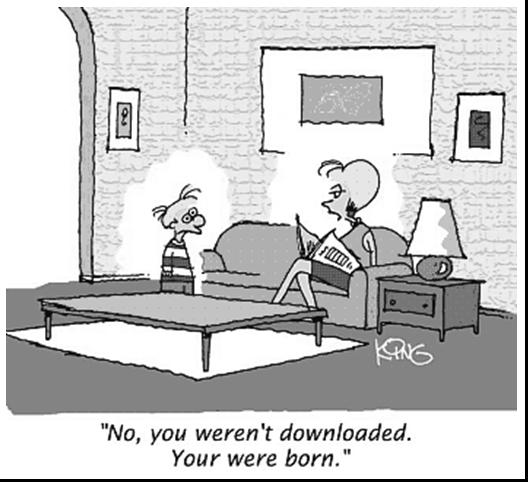
\includegraphics[width=0.4\textwidth]{./img/exemplo.jpg}\\
\small{Elaborado pelo autor.}
\end{figure}

Pode inserir v�rias figuras lado a lado tamb�m. Um exemplo est� reproduzido a seguir.

\begin{figure}[H]
  \centering
  \caption{Canal cl�ssico cuja obten��o da capacidade erro-zero � n�o-trivial.}
  \subfloat[\ ]{\label{fig:exG5}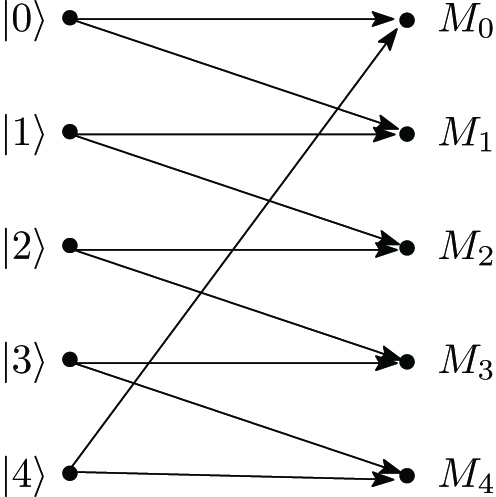
\includegraphics[width=0.3\textwidth]{./img/001}}
  \hspace{0.5cm}
  \subfloat[\ ]{\label{fig:exG52}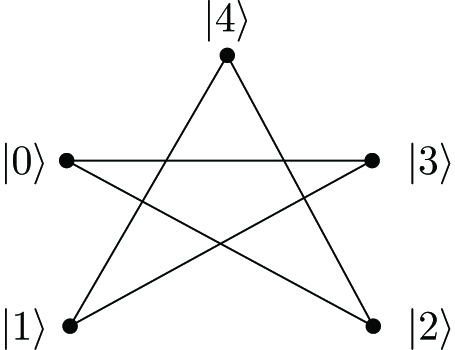
\includegraphics[width=0.3\textwidth]{./img/002}}
  \hspace{0.5cm}
  \subfloat[\ ]{\label{fig:exG53}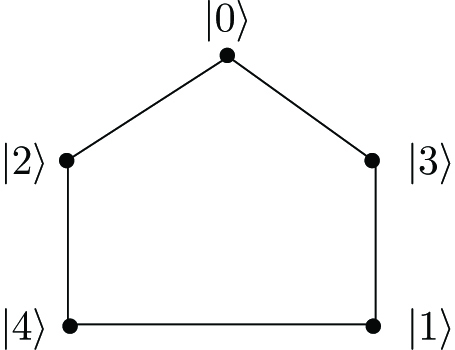
\includegraphics[width=0.3\textwidth]{./img/003}}\\
  \small{Elaborado por Bacon}
\end{figure}





\section{Refer�ncias Bibliogr�ficas no Padr�o ABNT}


\chapter{T�tulo do Quarto Cap�tulo}


Vivamus ultricies tincidunt lacus ut pharetra. Sed fringilla hendrerit tempus. Suspendisse potenti. Cras hendrerit tortor ac est condimentum pellentesque. Morbi pretium lectus nec sapien laoreet eu malesuada diam adipiscing. Aliquam nisl ipsum, fermentum ut aliquam nec, varius sit amet nisi. Pellentesque interdum cursus malesuada. Vestibulum ante ipsum primis in faucibus orci luctus et ultrices posuere cubilia Curae; Nullam malesuada bibendum tortor, ut bibendum lorem varius eu. In eros orci, volutpat ut facilisis sit amet, commodo quis nulla.

Sed lectus metus, mollis nec vulputate id, imperdiet eget urna. Nam ut dolor at metus venenatis suscipit et in ligula. In hac habitasse platea dictumst. Mauris scelerisque dolor sed nisl mattis accumsan. Aliquam vulputate placerat feugiat. Pellentesque faucibus neque mi. Etiam porttitor varius tempus. Mauris varius porttitor posuere. Pellentesque iaculis imperdiet lobortis. Sed vulputate purus nec felis rutrum molestie.


\section{Algoritmos}




Nunc at fringilla dui. Pellentesque id tortor eu libero auctor rhoncus id vel velit. Duis auctor laoreet turpis, sed commodo tellus sollicitudin sit amet. Phasellus quis purus consectetur turpis hendrerit pretium eget in velit. Cras dignissim est vel mi malesuada a imperdiet velit condimentum. Vivamus ultrices diam non urna aliquet hendrerit. Sed lobortis, mauris quis egestas ullamcorper, nunc nulla auctor nulla, eu rutrum velit velit in nulla. Etiam lectus augue, pellentesque et porta at, pharetra id lectus. Duis eleifend eleifend mauris, nec mollis mauris vehicula nec. Nam sed ipsum ut massa lacinia vestibulum. Duis vitae sapien a lectus aliquam luctus eget sit amet nunc. Etiam a ipsum auctor tortor condimentum consectetur. Aliquam vestibulum libero sit amet nulla auctor aliquet. Sed laoreet imperdiet tellus non vulputate. Vivamus tristique ipsum vel metus venenatis in laoreet tortor hendrerit. Suspendisse potenti. Aenean tincidunt molestie libero sit amet porttitor. Class aptent taciti sociosqu ad litora torquent per conubia nostra, per inceptos himenaeos.





Cras nec quam mi, ut mattis ante. Lorem ipsum dolor sit amet, consectetur adipiscing elit. Sed fringilla auctor dictum. Nam hendrerit sapien sed massa consequat rutrum. Nullam congue, augue sed commodo malesuada, lectus nulla mollis magna, eget semper risus nisl eget elit. Duis vitae hendrerit massa. In a odio nunc, sit amet mollis dolor. In accumsan suscipit dui, a vestibulum diam condimentum ullamcorper. Etiam ut quam arcu, ac tristique ante. Vestibulum imperdiet elit non ante tristique accumsan. Donec vulputate fringilla tempor. Proin porttitor nisi nisi. Fusce vel ullamcorper orci. Lorem ipsum dolor sit amet, consectetur adipiscing elit. 

Vivamus ultricies tincidunt lacus ut pharetra. Sed fringilla hendrerit tempus. Suspendisse potenti. Cras hendrerit tortor ac est condimentum pellentesque. Morbi pretium lectus nec sapien laoreet eu malesuada diam adipiscing. Aliquam nisl ipsum, fermentum ut aliquam nec, varius sit amet nisi. Pellentesque interdum cursus malesuada. Vestibulum ante ipsum primis in faucibus orci luctus et ultrices posuere cubilia Curae; Nullam malesuada bibendum tortor, ut bibendum lorem varius eu. In eros orci, volutpat ut facilisis sit amet, commodo quis nulla.





% Refer�ncia segundo o padr�o ABNT
% Edite este arquivo e inclua suas refer�ncias segundo a nota��o do Bibtex
\bibliography{ref}



\end{document}